\section{Support for Customization in PSWare}
\label{sec:flexibility}
An important feature of PSWare is that it can be customized. To support customization, PSWare uses a flexible layered architecture. In this way, developers can customize different layers without affecting each other. Moreover, multiple event processing strategies may be dynamically used during the runtime. In this section, we how such customization can be done at different layers. These layers consist different aspects of a complete event-based system, including, event detection, event delivery and event subscription.

\subsection{Customizable Event Definition}
It is a common scenario for the applications to define extra event attributes that have domain-specific meanings. For example, in an application which requires reliable communication, we might want to define a probability value which specifies the threshold for the message loss. Then in the middleware framework, this number should be used during the actual communication.

The simplest way to pass some domain-specific information to the middleware is to modify the System event. As discussed in Section \ref{sec:design}, the System event is used like a device driver that represents the primitive events collected by the system. Internally, this event is specified in a header file and can be modified to suit different applications. The essential steps are as follows:
\begin{enumerate}
\item Modify 'SystemEvent.h' and add necessary attributes for the system event
\item Use 'psware gen' to generate the necessary constant values for accessing the new attribute in the middleware runtime environment
\item Modify the middleware framework so that the attributes can be used
\item Use the new attributes in the actual event definition
\end{enumerate}

We will illustrate these steps through an application scenario. Suppose the middleware developer has implemented a message retransmission mechanism for the event delivery and matching functions to make the application more reliable. Then the application developers can specify a parameter indicating the desired reliability for the events they define. The new 'SystemEvent.h' will look like in Listing \ref{lst:SystemEventProbability}.

\begin{lstlisting}[caption=Customized system event, label=lst:SystemEventProbability]
typedef struct {
	uint16_t nodeID;
	uint16_t time;
	float probability;
} SystemEvent;
\end{lstlisting}

Once the new probability attribute is defined, we need to generate some necessary constant values for accessing the attribute. The tool for generating the constants is 'psware gen'. It will parse the event header files and output some macro values. After that, the middleware can access the attribute with the code fragment shown in Listing \ref{lst:SystemEventProbabilityAccess}. In this piece of code, we first obtain the system event through the EventInstance API. Then we obtain the probability value by accessing the correct attribute. Note that SystemEvent, SystemEvent\_probability are generated constant values for accessing the events and their attributes.

\begin{lstlisting}[caption=Customized system event, label=lst:SystemEventProbabilityAccess]
EventInstanceInfo * systemPtr = call EventInstance.getEventInstance(SystemEvent);
float probability = (float)systemPtr->content[SystemEvent_probability];
\end{lstlisting}

The event probability can then be further defined through event definition. To reuse the event definition in Listing \ref{lst:rooms}, now if the user wants to add a parameter to indicate the reliability, he may insert a statement at Line \ref{lst:reliability:def} which defines the global reliability parameter.

\begin{lstlisting}[caption=Example of event definition with reliability, label=lst:reliability]
Event SimpleEvent {
	int temp=System.temp;
	int id=System.id;
	int time=System.time;
	System.reliability = 1.0; (* \label{lst:reliability:def} *)
} where {
	temp > 30
}
Event CompEvent {
} on {
	SimpleEvent e1 and
	SimpleEvent e2
} where {
	e1.Location="A" and
	e2.Location="B" and
	e2.time-e1.time=600
}
\end{lstlisting}

Once the parameter is defined. The information will be passed to the middleware and the corresponding code fragment in Listing \ref{lst:SystemEventProbabilityAccess} will work as expected.

\subsection{Customizable Event Detection}
Event detection is the heart of an event-based system. In PSWare, we can easily customize event detection on the event detection layer. Since PSWare uses a type-based event model to support composite event, event detection can also be customized according to the event types. The customization takes the following steps:
\begin{enumerate}
\item Define some domain-specific event types that requires specific event detection methods
\item Generate the necessary constant values for accessing the new attribute in the middleware runtime environment
\item Implement the specific event detection methods in the middleware
\end{enumerate}

We demonstrate the steps through a simple example, iTED. iTED is a variation of the TED \cite{lai:ted} algorithm, the default event detection algorithm in PSWare. Different from TED, iTED is customized for indoor monitoring application where the events are first fused in each monitored room. Then the results are further fused for global event detection. For simplicity, we assume each sensor node is equipped with a room ID and there maybe more than one fusion points in each room. However, all fusion points are selected in advance and will remain unchanged. The room ID can either be pre-deployed in the sensor nodes' program or be obtained using localization methods and more sophisticated fusion point selection methods may be implemented by extending some components discussed here.

\begin{figure}
\centering
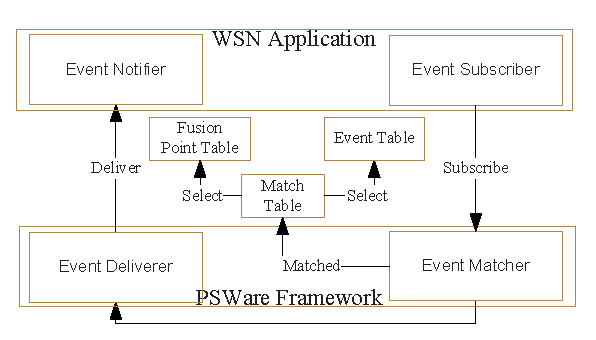
\includegraphics[width=.8\textwidth]{ted-architecture}
\caption{iTED over PSWare}
\label{fig:ted-architecture}
\end{figure}

Figure \ref{fig:ted-architecture} shows an overall diagram on how iTED interacts with PSWare. To implement iTED in PSWare, we need three key components:
\begin{enumerate}
\item Fusion point table: each sensor node updates this table in order to find the fusion point.
\item Event table: each sensor node maintains this table in order to decide if a given detected event should be forwarded to the fusion point.
\item Event matcher: a component that implements the event matching interface as discussed in Section \ref{sec:model}, Listing \ref{lst:pswareEventMatcher}.
\end{enumerate}

The first step is to add a new attribute, roomID, to our system event. This has already been discussed in the previous sub-section in Listing \ref{lst:SystemEventProbability} and we will skip it here. The only difference is the new attribute here will be of 'int' type instead of 'float' type.

Our first component, the fusion point table maintained by each sensor node \(v'_n\in V'\) is denoted as \(table_r\). It contains the following data:
\begin{itemize}
\item	Hop count (\(hop_n\)): the number of hops to reach the fusion point
\item	Parent (\(parent_n\)): the next hop to that fusion point
\end{itemize}

The procedure for updating fusion point table is shown in Procedure \ref{algo:table_r}. Note that we make use of the roomID to filter the messages.
\begin{algorithm}
\begin{algorithmic}
\REQUIRE \(v_n\rightarrow msg_r\)
	\FOR {each entry \(t'\) in \(msg_r\)}
		\IF {\NOT exists \(t'\rightarrow fid_n\) in \(table_r\)}
			\STATE \(addTo(table_r, t')\)
		\ENDIF
		\FOR {each entry \(t\) in \(table_r\)}
			\IF {\(t\rightarrow roomID = t'\rightarrow roomID\)}
				\IF {\(t'\rightarrow hop_n < t\rightarrow hop_n\)}
					\STATE \(t\rightarrow hop_n \gets t\rightarrow hop_n+1\)
					\STATE \(t\rightarrow parent_n \gets v_n\)
				\ENDIF
			\ENDIF
		\ENDFOR
	\ENDFOR
	\IF {self is fusion point \AND \NOT exists \(self\rightarrow id\) in \(table_r\)}
		\STATE \(addTo(table_r, (self\rightarrow id, 0, self\rightarrow id))\)
	\ENDIF
	\STATE \(msg_r \gets table_r\)
	\STATE \(periodically\_broadcast(msg_r)\)
\end{algorithmic}
\caption{Fusion point table exchange}
\label{algo:table_r}
\end{algorithm}

The second and the last component, the event table and the event matcher are closely related. Each sensor node will maintain an event table which is denoted as \(table_e\). The event table contains information for each event type \(e_n\in E\) as follows:
\begin{itemize}
\item Event type ID (\(e_n\)): the ID which is assigned to each event type
\item Fusion point for the event (\(fusion_n\)): the fusion point at which the event is mostly likely to be detected at the lowest cost.
\item Fusion cost (\(cost_n\)): the fusion cost for event type \(e_n\)
\end{itemize}

In addition, each fusion point \(v'\in V'\) will maintain another table, the event matching \(table_m\) for the purpose of matching events. \(table_m\) contains the following fields:
\begin{itemize}
\item Event type ID (\(e_n\)): the ID of the event type
\item Event instance ID (\(i\)): the \(i\)th event instance of event type \(e_n\) (we use \(e_n^i\) to denote such an instance of event)
\item Source node (\(v_n^i\)): the node which forwarded \(e_n^i\) to the fusion point
\item Event timestamp (\(t_n^i\)): the timestamp when the event \(e_n^i\) is detected
\item Detection cost (\(cost_n^i\)): the cost for detecting event \(e_n^i\)
\end{itemize}

First, each node \(v_n\) periodically broadcasts messages \(msg_r\) which is its \(table_r\). If the node itself is a fusion point, then it will add itself in \(table_r\) and broadcast the message. The procedure is shown in Procedure \ref{algo:table_r}. In addition to \(msg_r\), each \(v'_k\in V'\) will periodically advertise its \(table_m\) by broadcasting \(msg_m\) so that other sensor nodes can construct their \(table_e\) with Procedure \ref{algo:table_e}.

\begin{algorithm}
\begin{algorithmic}
\REQUIRE \(v'_k\rightarrow msg_m\)
	\FOR {each entry \(t'\) in \(msg_m\)}
		\IF {\NOT exists \(t'\rightarrow e_n\) in \(table_e\)}
			\STATE \(addTo(table_e, (t'\rightarrow e_n, 1, v'_k, t'\rightarrow cost_n^i+table_r\rightarrow hop_k))\)
		\ENDIF
		\FOR {each entry \(t\) in \(table_e\)}
			\IF {\(t\rightarrow e_n = t'\rightarrow e_n\)}
				\IF {\(t'\rightarrow cost_n^i+table_r\rightarrow hop_k < t\rightarrow cost_n\)}
					\STATE \(t\rightarrow cost_n \gets t'\rightarrow cost_n^i+table_r\rightarrow hop_k\)
					\STATE \(t\rightarrow fusion_n \gets v'_k\)
				\ENDIF
			\ENDIF
		\ENDFOR
	\ENDFOR
	\IF {self is fusion point}
		\STATE \(msg_m \gets table_m\)
		\STATE \(periodically\_broadcast(msg_m)\)
	\ENDIF
\end{algorithmic}
\caption{Event table exchange}
\label{algo:table_e}
\end{algorithm}

The construction of \(table_m\) will take place when the event instance \(e_n^i\) is detected and forwarded to a fusion point \(v'_n\). We will discuss how forwarding could be done in the next subsection.

When an event \(e_n^i\) is matched at node \(v_k\), node will use \(table_r\) and \(table_e\) to decide how to forward the detected event to the fusion points so that higher level events can be matched. In case the fusion point for event type \(e_n\) has not been decided, the node will forward the event to some of its closet fusion points  according to iTED. Upon the reception of \(e_n^i\) from \(v_k\), the fusion point will first update its own \(table_m\). Then it will check if there is any composite event \(e_{comp}\) which uses \(e_n\) and another event \(e_j\) as its sub-event (\(e_{comp}=comp(e_n, e_j)\)). If there is, then \(e_j\) will be used upon 'selectSubevent'.

\begin{algorithm}
\begin{algorithmic}
\REQUIRE \(e_n^i\) matched by \(v_k\) with cost: \(cost_n^i\)
	\STATE \(addTo(table_m, (e_n, e_n^i, v_k, now(), cost_n^i))\)
	\FOR {each \(e_j\) in \(E\)}
		\IF {\(\exists r\in R\) \AND \(r=e_{comp}=comp(e_n, e_j)\)}
			\FOR {each \(e_j^k\) in \(table_m\)}
				\IF {\(comp(e_n^i, e_j^k)=true\)}
					\STATE \(addTo(table_m, (e_{comp}, e_{comp}^i, self, now(), cost_n^i+cost_j^k))\)
					\STATE \(detected(e_{comp})\)
				\ENDIF
			\ENDFOR
		\ENDIF
	\ENDFOR
\end{algorithmic}
\caption{Event matching}
\label{algo:eventmatching}
\end{algorithm}

If \(e_{comp}\) has been successfully detected by the underlying event matcher, then Procedure \ref{algo:eventmatching} will be executed so that \(table_m\) is updated accordingly and iTED may reduce the energy cost for future event detection. Note that Procedure \ref{algo:eventmatching} will make use of the APIs in Listing \ref{lst:pswareAPI} since it needs to query the event relations.

\subsection{The Event Delivery Layer}
After the subscribed event is detected, it needs to be delivered to the user. In many applications, this is done via the underlying routing protocols such as CTP provided by TinyOS. This is also the case for the default event delivery in PSWare. However, in some applications, this may not be a case. For example, in an intelligent transportation system, the events may be delivered to mobile vehicles. In this subsection, we show how PSWare can achieve the flexibility in event delivery through several examples in ITS.

We choose ITS as an example because different event types in this application may require different event delivery strategies and that is why the flexibility in event delivery is of particular importance. The event types in ITS may include:
\begin{itemize}
\item Emergency: events that represent urgent incidents. Examples of this type of events include car accidents and urgent road maintenance. These events probably need to be delivered to all nearby vehicles when occurred.
\item Driver's information: events that provide assistant information to the drivers. Examples include congestion information and whether information These events are usually not considered as urgent and may be delivered in carry-and-forward fashion \cite{cartel}.
\end{itemize}

\begin{figure}
\centering
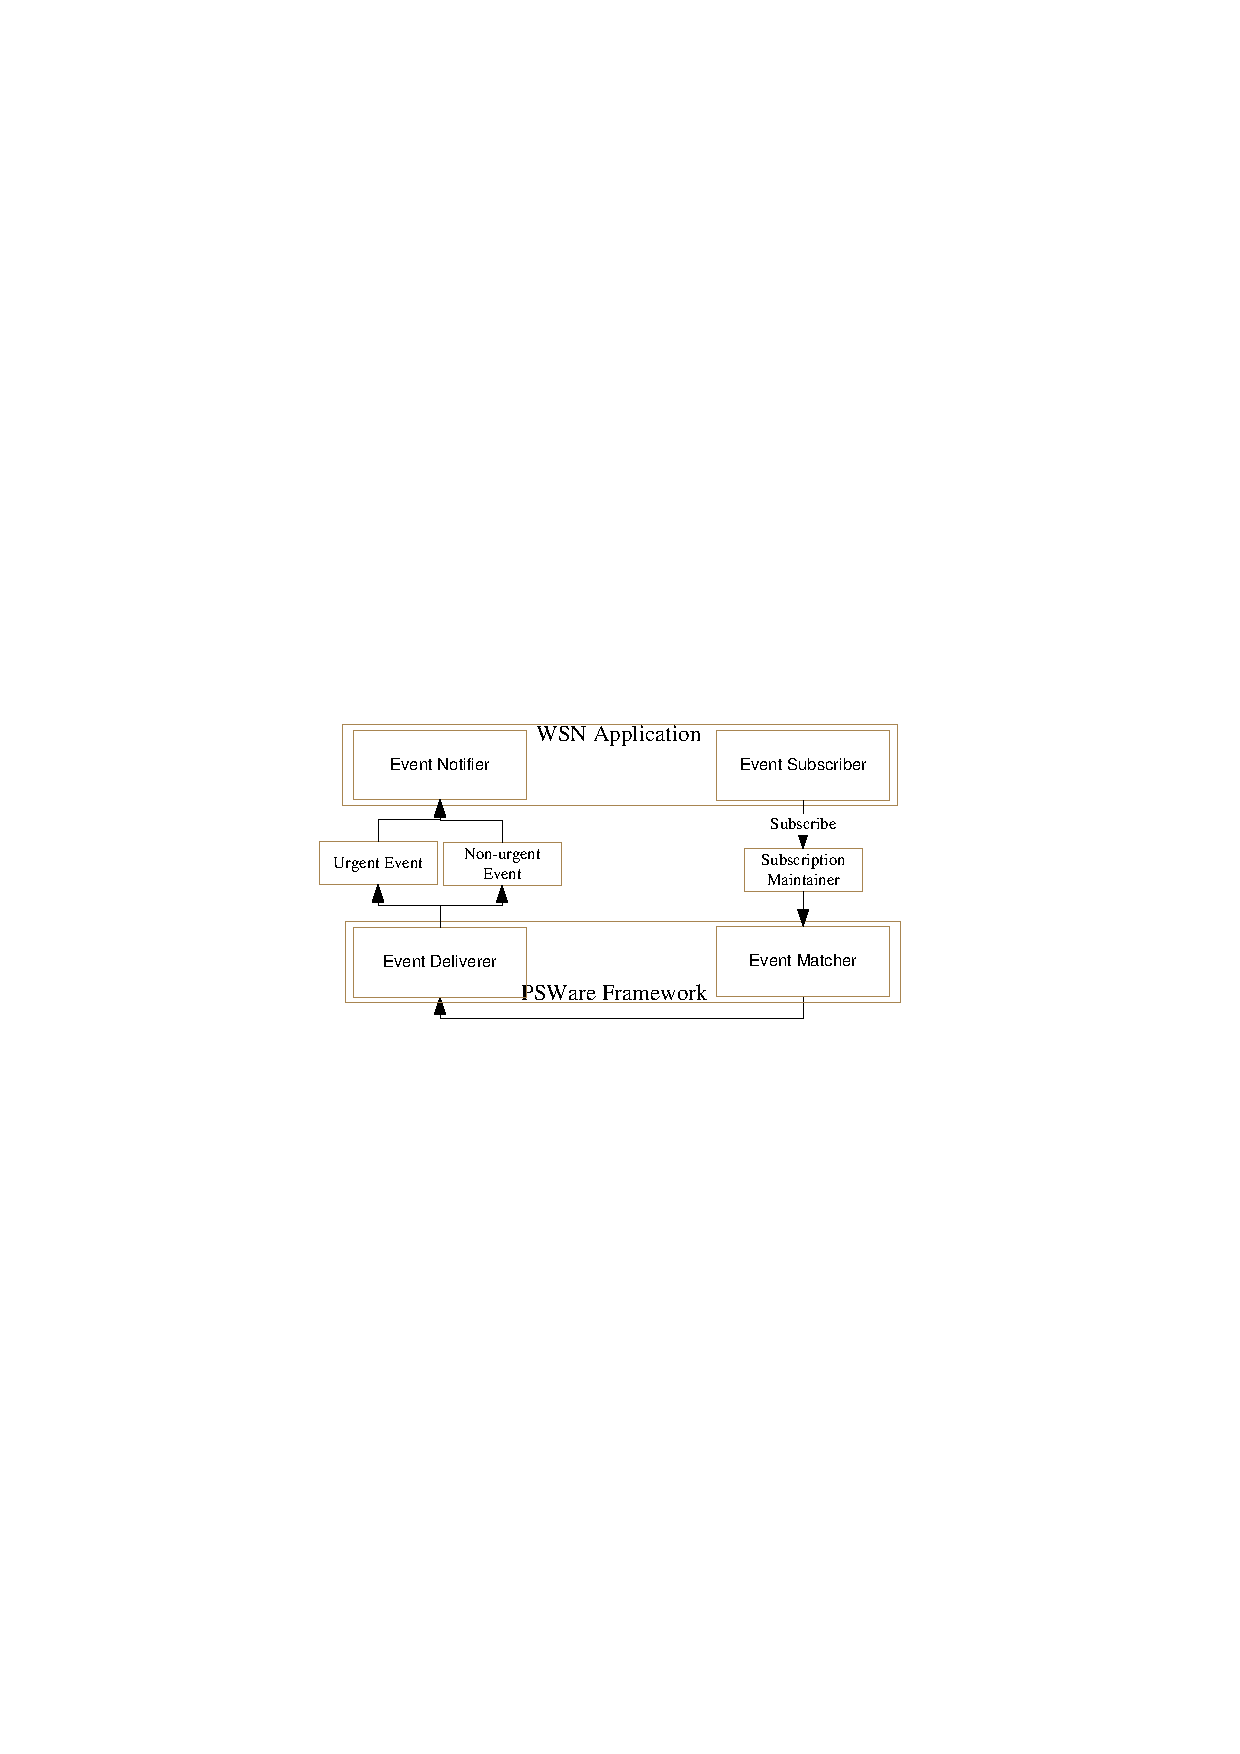
\includegraphics[width=.8\textwidth]{its-delivery}
\caption{Type-based event delivery}
\label{fig:its-delivery}
\end{figure}

The overall architecture for ITS event delivery over PSWare is shown in Figure \ref{fig:its-delivery}. A key difference in this architecture is the introduction of multiple event deliverer. Upon the signaling of 'eventDeliver' in Listing \ref{lst:pswareEventMatcher}, the middleware developer can first query the event type by using the APIs in Listing \ref{lst:pswareAPI}. Then if the event type is accident, it will be immediately delivered to the nearby vehicles. Otherwise, a carry-and-forward mechanism will be used to deliver the event.
